\documentclass[12pt]{article}
\usepackage[utf8]{inputenc}
\usepackage{float}
\usepackage{amsmath}
\usepackage{tikz}

\usepackage[hmargin=3cm,vmargin=6.0cm]{geometry}
%\topmargin=0cm
\topmargin=-2cm
\addtolength{\textheight}{6.5cm}
\addtolength{\textwidth}{2.0cm}
%\setlength{\leftmargin}{-5cm}
\setlength{\oddsidemargin}{0.0cm}
\setlength{\evensidemargin}{0.0cm}

%misc libraries goes here



\begin{document}

\section*{Student Information } 
%Write your full name and id number between the colon and newline
%Put one empty space character after colon and before newline
Full Name : Göktuğ Ekinci \\
Id Number : 2380343 \\

% Write your answers below the section tags
\section*{Answer 1}
\subsection*{a)}
\begin{figure}[H]
	\centering
	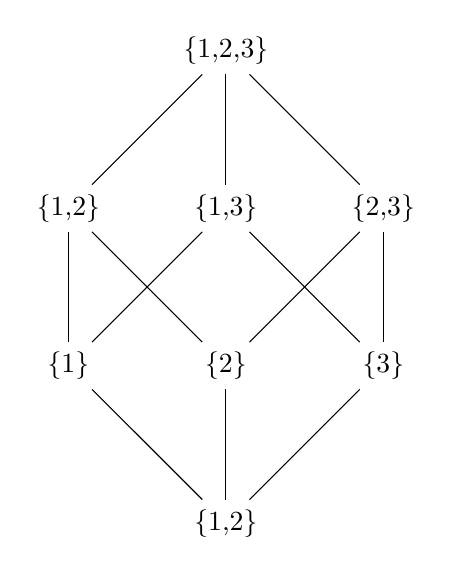
\begin{tikzpicture}
	
	\node[draw=none,fill=none] (e) at (0, 0)     {\{1\}};
	\node[draw=none,fill=none] (b) at (0, 2)     {\{1,2\}};
	\node[draw=none,fill=none] (a) at (2, 4)     {\{1,2,3\}};
	\node[draw=none,fill=none] (c) at (2, 2)     {\{1,3\}};
	\node[draw=none,fill=none] (d) at (4, 2)     {\{2,3\}};
	\node[draw=none,fill=none] (f) at (2, 0)     {\{2\}};
	\node[draw=none,fill=none] (g) at (4, 0)     {\{3\}};
	\node[draw=none,fill=none] (h) at (2, -2)     {\{1,2\}};

	
	\path[-] (a) edge (b);
	\path[-] (a) edge (c);
	\path[-] (a) edge (d);
	\path[-] (b) edge (e);
	\path[-] (b) edge (f);
	\path[-] (c) edge (e);
	\path[-] (c) edge (g);
	\path[-] (d) edge (f);
	\path[-] (d) edge (g);
	\path[-] (e) edge (h);
	\path[-] (f) edge (h);
	\path[-] (g) edge (h);
	
	
	
	\end{tikzpicture} 
	\caption{Hasse Diagram}	
	\label{fig:g2}
\end{figure}
\subsection*{b)}
Yes.
\subsection*{c)}
{1,2,3}
\subsection*{d)}
\O
\subsection*{e)}
Yes.
\subsection*{f)}
Yes.
\subsection*{g)}
LUBs of \{1\} are \{1,2\} and \{1,3\}. LUBs of \{3\} are \{1,3\} and \{2,3\}.
\section*{Answer 2}
\subsection*{a)}
Sum of all degrees is the twice of edge number. There are 7 edges, so:\\
7 $\times$ 2 = 14 is the sum of all degrees.
\subsection*{b)}
In adjacency matrix, nothing will be filled but edges. Since if node a has an edge with b, b also has an edge with a. Number non-zero entries in adjacency matrix is going to be equal to edge $\times$ 2, which is 14.
\subsection*{c)}
Every edge has to points, or two nodes we can say. So, number of non-zero entries in incidence matrix will be equal to edge $\times$ 2, which is 14.
\subsection*{d)}
\begin{figure}[H]
	\centering
	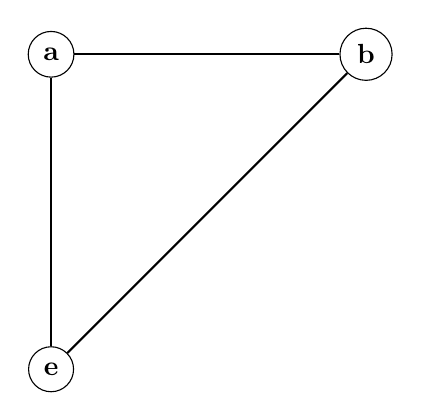
\begin{tikzpicture}
	
	\node[shape=circle,draw=black] (a) at (0, 4)     {\textbf{a}};
	\node[shape=circle,draw=black] (b) at (4, 4)     {\textbf{b}};
	\node[shape=circle,draw=black] (e) at (0, 0)     {\textbf{e}};
	
	\path[-, thick] (a) edge (b);
	\path[-, thick] (a) edge (e);
	\path[-, thick] (b) edge (e);
	
	\end{tikzpicture} 
	\caption{Complete subgraph of G}	
	\label{fig:g2}
\end{figure}
\subsection*{e)}
No, to make this a bipartite graph, we have to remove the edges between c,d and b,e.
\begin{figure}[H]
	\centering
	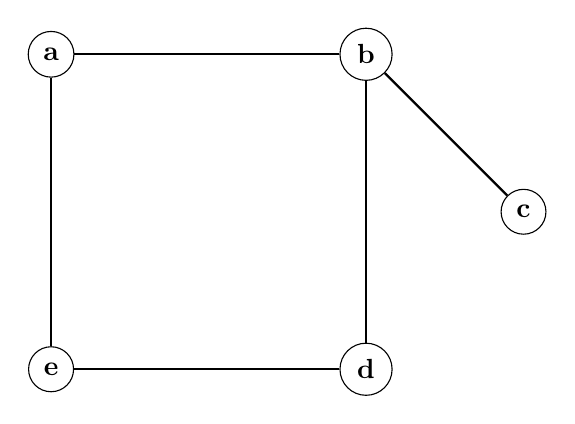
\begin{tikzpicture}
	
	\node[shape=circle,draw=black] (a) at (0, 4)     {\textbf{a}};
	\node[shape=circle,draw=black] (b) at (4, 4)     {\textbf{b}};
	\node[shape=circle,draw=black] (c) at (6, 2)     {\textbf{c}};
	\node[shape=circle,draw=black] (d) at (4, 0)     {\textbf{d}};
	\node[shape=circle,draw=black] (e) at (0, 0)     {\textbf{e}};
	
	\path[-, thick] (a) edge (b);
	\path[-, thick] (a) edge (e);
	\path[-, thick] (b) edge (c);
	\path[-, thick] (b) edge (d);
	\path[-, thick] (d) edge (e);
	
	\end{tikzpicture} 
	\caption{Bipartite form of G}	
	\label{fig:g2}
\end{figure}

\subsection*{f)}
There are three possibilities for the edges in this situation. They have 2 points and they can be directed to one,the other or both. Since there are 7 edges there are $3^7$ possibilities.
\subsection*{g)}
We have to go through every edge maximum once. Longest simple path can be like this: d,c,b,e,b,a,e. We visit 7 nodes.
\subsection*{h)}
There is just one connected component for this graph, which is G itself. There is no disconnected nodes to G.
\subsection*{i)}
No, there is not.
\subsection*{j)}
Yes, there is. We can count the path that I mentioned in (g) as a Euler path.
\subsection*{k)}
Yes, there is a Hamilton Circuit in this graph which can be the outer circle. a,b,c,d,e. This path visit every node just once.
\subsection*{l)}
The circuit that I mentioned in (k) can be counted as a Hamilton Path, so yes.

\section*{Answer 3}
To show these are isomorphic, we should define a function that matches every node from one graph to the other, and this function must be onto and one-to-one. Also, this function should match the nodes that have same adjacents and edges. So, function f must have the following properties: \\
f(a) = a', f(b) = c'\\
f(c) = e', f(d) = g'\\
f(e) = b', f(f) = h'\\
f(g) = d', f(h) = f'\\
As you can see f is onto and one-to-one. It also matches the same roles of nodes of two graphs.

\section*{Answer 4}
    
\begin{table}[h!]
\begin{center}
\begin{tabular}{|l|l|l|l|l|l|l|l|l|l|l|l|}
\hline
visit / nodes & a & b                & c                & d                & e                & f                & g                & h                & i                & j                & k                \\ \hline
--          & 0 & $\infty$ & $\infty$ & $\infty$ & $\infty$ & $\infty$ & $\infty$ & $\infty$ & $\infty$ & $\infty$ & $\infty$ \\ \hline
a             & 0 & 3                & $\infty$ & $\infty$ & 5                & $\infty$ & $\infty$ & 4                & $\infty$ & $\infty$ & $\infty$ \\ \hline
b             & 0 & 3                & 5                & $\infty$ & 5                & 10               & $\infty$ & 4                & $\infty$ & $\infty$ & $\infty$ \\ \hline
h             & 0 & 3                & 5                & $\infty$ & 5                & 9                & $\infty$ & 4                & 6                & $\infty$ & $\infty$ \\ \hline
e             & 0 & 3                & 5                & $\infty$ & 5                & 9                & $\infty$ & 4                & 6                & $\infty$ & $\infty$ \\ \hline
c             & 0 & 3                & 5                & 8                & 5                & 7                & 11               & 4                & 6                & $\infty$ & $\infty$ \\ \hline
i             & 0 & 3                & 5                & 8                & 5                & 7                & 11               & 4                & 6                & 12               & $\infty$ \\ \hline
f             & 0 & 3                & 5                & 8                & 5                & 7                & 11               & 4                & 6                & 10               & $\infty$ \\ \hline
d             & 0 & 3                & 5                & 8                & 5                & 7                & 11               & 4                & 6                & 10               & 10               \\ \hline
k             & 0 & 3                & 5                & 8                & 5                & 7                & 11               & 4                & 6                & 10               & 10               \\ \hline
\end{tabular}
\end{center}
\end{table}
\begin{center}
If we backtrack the table, we see that the shortest path is a,b,c,f,j.
\end{center}
\section*{Answer 5}
\subsection*{a)}
I prefer to use Kruskal's Algorithm:
Order of added edges are ab, ce, cf, ad, bc

\subsection*{b)}
\begin{figure}[H]
	\centering
	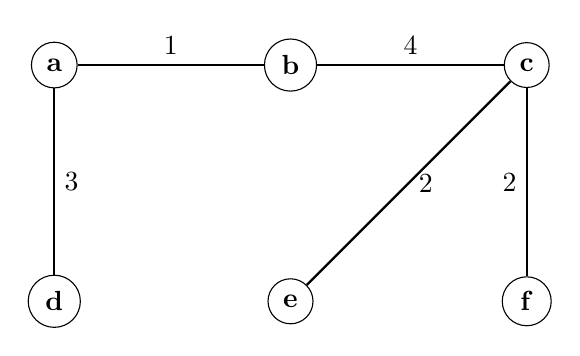
\begin{tikzpicture}
	
	\node[shape=circle,draw=black] (a) at (0, 3)     {\textbf{a}};
	\node[shape=circle,draw=black] (b) at (3, 3)     {\textbf{b}};
	\node[shape=circle,draw=black] (c) at (6, 3)     {\textbf{c}};
	\node[shape=circle,draw=black] (d) at (0, 0)     {\textbf{d}};
	\node[shape=circle,draw=black] (e) at (3, 0)     {\textbf{e}};
	\node[shape=circle,draw=black] (f) at (6, 0)     {\textbf{f}};
	
	\path[-, thick] (a) edge node[above]{1} (b);
	\path[-, thick] (b) edge node[above]{4} (c);
	\path[-, thick] (a) edge node[right]{3} (d);
	\path[-, thick] (c) edge node[right]{2} (e);
	\path[-, thick] (c) edge node[left]{2} (f);
	
	\end{tikzpicture} 
	\caption{Minimum spanning tree of Q5}	
	\label{fig:g5}
\end{figure}
\subsection*{c)}
No, it is not. We can choose the same weight edges in different order. Here is two example;\\
\{ab,cf,fe,ad,bc\} and \{ab,ce,cf,ad,bc\}

\section*{Answer 6}
\subsection*{a)}
Number of vertices: 13\\
Number of edges: 12\\
Height: 4
\subsection*{b)}
Post Order: w,s,m,t,q,x,n,y,u,z,v,r,p
\subsection*{c)}
Inorder: s,w,q,m,t,p,x,u,n,y,r,v,z
\subsection*{d)}
Pre Order: p,q,s,w,t,m,r,u,x,y,n,v,z
\subsection*{e)}
No, y has only one child. This is a contradiction with the definition of full binary tree.



\end{document}